\subsection{Testbenches}

For each module developed a corresponding self testing testbench is provided. Most of the tests are takes benefit of the function {\bf assertEqual(actual, expected) } defined in the assert.vhd file.

The first three testbench are selftesting and are considered successfull if no assertions with severity {\bf warning} fails. Assertions with severity {\bf note} is included in order for readability when tests are failing.

\subsubsection{Running tests}
The test can be run in Modelsim by following the following procedure.


\begin{enumerate}
\item Open the ISE projected located at:  \\ {\bf system/system/pcores/mips\_multi\_cycle\_v1\_00\_a/devl/projnav/mips\_multi\_cycle.xise}
\item Open the simulation tab located at the left of the screen. 
\item Select the testbench to run.
\item Open the ModelSim application from the menu under the navigator view. 
\item All selftesting testbenches should automatically run
\item The result should appear in the console. 
\end{enumerate}

\subsubsection{Testbench - ALU Control Unit}
This testbench, {\bf alu\_control\_tb.vhd}, verifies that the ALU Control state machine is behaving acording to specifications. It has one test case for each of the possible outputs.
\subsubsection{Testbench - Control Unit}
This testbench, {\bf control\_unit\_tb.vhd} , makes sure that the Control Unit asserts the correct signal for the given opcode. It also tests the states of state machines.
\subsubsection{Testbench - Processor}
The {\bf processor\_tb.vhd} testbench tests each of the implemented MIPS instructions in isolation. Later tests depends on some of the instructions tested in the start of the file.
\subsubsection{Testbench - Toplevel}

\paragraph{Description}

This testbench was provided with the startup code and was used to confirm that the processor was able to run a program. The testbench is not a selftesting testbench and must be verified manually. It uses approximetly 108 cycles to load a data and program into the data and instruction memory, then is starts up the and lets it run the program.

An assembly equivalent of the program can be found in attachment \ref{sec:assembly}.
In summary the program loads 2 and 10 into register \$1 and \$2, adds them into \$3 and stores the value 12 into memory location 5, then it jumps over a couple of instrutions and stores 12 at location 6 and 7. At the end it loads a big immidiate value into \$3, stores it at location 8, adds 2 to the register stores it to location 9 and loops the add and store instruction. The last store instruction at location 10 should not be executed.

\paragraph{Expected results}
\label{sec:exp-res}
The expected result of running this program is the following memory layout. 
\begin{table}[h]
	\label{tab:exp-res}
	\begin{tabular}{|l|c|c|c|c|c|c|c|c|c|c|c|}
		\hline
		Address &  0 &  1 &  2 &  3 &  4 &  5 &  6 &  7 &  8 &  9 & 10 \\
		\hline
		Value   &  0 &  2 & 10 &  0 & 0 & 12  & 12 & 12 & 393216 & 393216 + i*2 & 0\\
		\hline
	\end{tabular}
	\caption{Expected memory layout}
\end{table}

\paragraph{Actual results}
This figure shows a screenshot from the ModelSim application. The processor correctness can be verified by comparing the second column with the above table.

\begin{figure}[h]
		\centerline{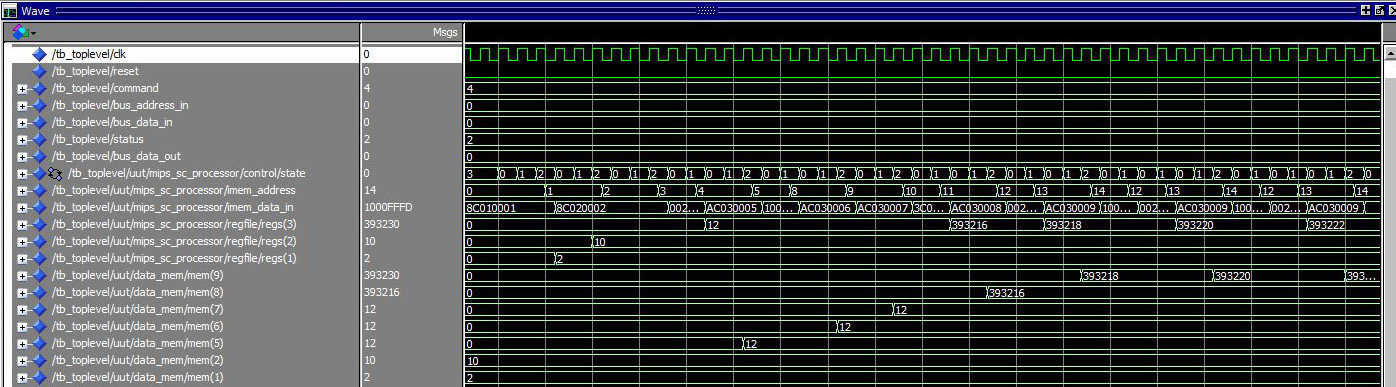
\includegraphics[width=550px]{figures/toplevel_tb_result}}
		\caption{Actual result}
\end{figure}

